\chapter{Techniques in Object Detection}

\section{Intersection over Union (IoU)}
\hspace{0.5cm}Intersection over Union (IoU) is the ratio of overlapping area of predicted bounding box and the ground truth bounding box over the total area of the both boxes. This metric allows us to evaluate how well the detector predict the bounding box of the object comparing to the ground truth ones.
\begin{figure}[h!]
    \centering
    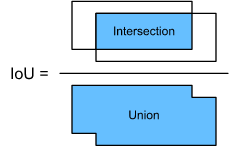
\includegraphics[scale=1]{Chapters/Fig/iou.png}
    \caption{Intersection over Union}
    \label{fig:iou}
\end{figure}\par

Ideally, if the predicted and the ground truth bounding boxes overlapped perfectly, the IoU would be equal to 1. However, in practical, the IoU greater than or equal to 0.5 is good to be used as threshold to determine the predicted bounding box is correct or not.
\section{Non-maximum Suppression}
\hspace{0.5cm}One the problems of Object Detection is that the algorithms may output multiple detections for the similar objects in multiple times. Non maximum suppression is an approach to make sure that a particular in the image scenes is identified only once.
\begin{figure}[h!]
    \centering
    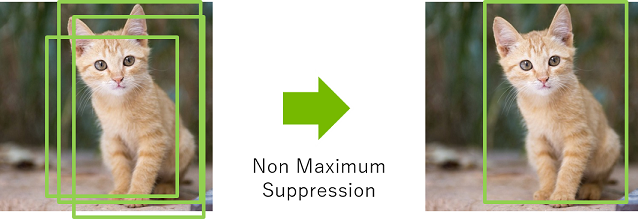
\includegraphics[width=0.8\textwidth]{Chapters/Fig/nms.png}
    \caption{Non Maximum Suppression}
    \label{fig:nms}
\end{figure}\par
For example, in the fig.\ref{fig:nms}, the algorithm may output a lot of detections with different confidence score (is a cat or not), then we run the these detections through our non maximum suppression which will get rid of boxes which have lower confidence scores and keep the only one bounding box with the highest confidence score.
\section{Anchor box}
\hspace{0.5cm}Anchor boxes are the set of predefined height and width bounding boxes which are used for assist the algorithm to be more certain in training and give the algorithms ability to detect more precise.
In real life, the bounding boxes of the objects are not arbitrary. Cars, vans have similar shapes of bounding box with larger width than height while pedestrian have an approximate aspect ratio of 0.41.
\begin{figure}[h!]
    \centering
    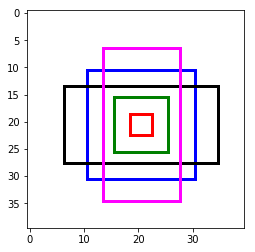
\includegraphics[scale=0.5]{Chapters/Fig/anchor_boxes.png}
    \caption{5 anchor boxes}
    \label{fig:ab}
\end{figure}\par
Moreover, instead of predicting absolute value of bounding boxes such as $x,y,w,h$ or $x1,y1,x2,y2$, the algorithms now only predict offsets corresponding to each of the anchor boxes . If we normalize the offset values in a fixed range, we can maintain the diversity, therefore, the initial training will be more stable.